\part{Preface}
\chapter{Introduction}
((To be written later))
\chapter{Problem Analysis}
\section{Problemstatement}
What are the theories and models behind the Rubik's cube and how can they be implemented in an application in order to solve the Rubik's cube?
\begin{itemize}
	\item Which mathematical models and theories describe the Rubik's cube?
	\item What is the origin of these theories and models and how have they evolved?
	\item How can the models and theories be implemented in an overall algorithm for solving the Rubik's cube?
	\begin{itemize}
		\item How can this algorithm be improved with respect to processing power?
	\end{itemize}
\end{itemize}
\section{Problem Limitations}
	%\documentclass{report}\begin{document}
\chapter{Origin of the Cube}

\myTop{In this chapter we will describe the history behind \erno{} and how he got the idea for the \rubik{} in order to get a better understanding of the \rubik{}. Furthermore we will look at the development and the problematics describing the patenting and legal issues regarding the cube. We will look at the patent to get a better understanding of the cubes made at that time. We will also decribe the development of the Upper- ans lower bound how it's has change throw time. The purpose of this chapter is to give the reader a basic understanding of the \rubik{}.}
\section{Ern\"{o} Rubik}
\erno{} is the inventor behind the world famous \rubik{}. He was born in Budapest, Hungary in 1944, his father was a flight engineer and his mother was a poet. He graduated from the Technical University in Budapest as an architectural engineer. After his graduation he stayed at the university to teach interior design.

In \myDate{}{1}{1975} Rubik applied for a patent for his invention in Hungary that was originally made to help his students. Two years later in 1977 he got the patent on the \mcube{}. This \mcube{} was actually the same cube as todays \rubik{}, he just named it differently. His \mcube{} should not be confused with the \mcube{} described in section \ref{sub:mcube}.
% Der er et spring fra Magic Cube til Rubiks Cube, som ikke beskrives

In the 1980's he became a professor and started the Rubik Studio, which employs a dozen people to design furniture and toys. 
Since the studios opening Rubik has produced several other toys, including Rubik's Snake. Most recently  the studio began developing computer games. 
He also became the president of the Hungarian Engineering Academy in 1990.The same year he created the International Rubik Foundation to support especially talented young engineers and industrial designers.

\begin{figure}
	\centering
		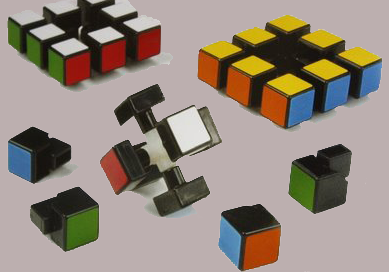
\includegraphics[scale=0.6]{input/pics/rubiks-cube.png}
	\caption{\myCaption{Figure of Rubik's Cube.}}
	\label{fig:rubiks-cube}
\end{figure}
 
\section{Rubik's Cube -- Magic Cube}

%In the 70s \erno{} was teaching Interior Design at Academy of Applied Arts and Crafts and he was trying to find a tool to help his students to understand three dimensional objects. As result he made the \mcube{} in 1974 and obtained a Hungarian patent HU170062. 
% Det ovenover er allerede beskrevet i forrige section

In the 1970's when \erno{} were teaching at the university he wanted to create a tool that would help his students to better understand tree-dimensional design. He wanted a design with blocks that could be moved individually, but also able to move several blocks at a time. Initially he attempted to do this with a cube held together by rubber bands. This failed. He then concluded after looking at a  Magic Puzzle (see chapter \ref{chap:recreationalMathematics}).
 that the pieces must hold each other in place. There by he created what was then called the \mcube{}. 

%Rubik described that some of the most important features behind the cube were that the parts of the cube stay together, which many other puzzles do not. He also pointed out that you can move several pieces at once. Also that it is three dimensional. 

In the end of 1970's a Hungarian Businessman showed the Magic Cube at the Nuremberg toy fair and made it popular in Europe. The company Ideal Toy bought exclusive rights for the Magic Cube, but changed the name of the cube to \rubik{} within a year in order to get trademark protection.

At that time there were also two others applying for patent for products similar to the \rubik{}.  One of them was an American man named Doctor Larry D. Nichols, and his cube was a 2x2x2 cube which was held together with magnets. See \ref{sec:nichols} .The other one who applied for patent was a Japanese man named Terutoshi Ishige. He applied for patent a year after Rubik. Terutoshi Ishige's cube was almost identically to the \rubik{}.

Ideal Toy Company were bought by CBS Toy Company in 1982 and the trademark surpassed with it, but they sold the rights to Rubik's Cube to Seven Towns which is a Toy Company in Great Britain, and they are still producing The Rubik's Cube today.

\section{The Nichols Cube Puzzle}
\label{sec:nichols}
Dr. Larry D. Nichols studied chemistry at DePauw University in Greencastle, Indiana, before moving to Massachusetts to attend Harvard Graduate School. 
He is a lifelong puzzle enthusiast and inventor who  began developing a twist cube puzzle with six colored faces in 1957. It was made of eight smaller cubes assembled to a 2x2x2 cube. The eight cubes were held together by magnets.

\begin{figure}[htb]
	\centering
		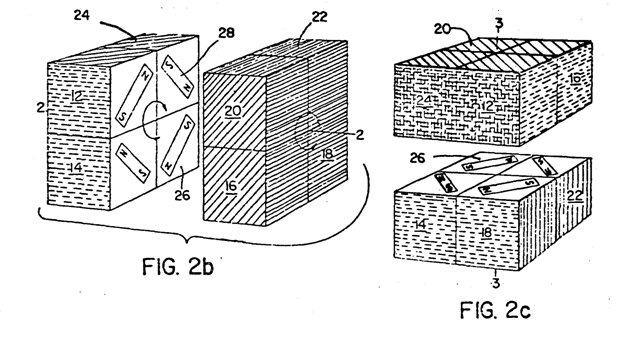
\includegraphics[scale=0.6]{input/pics/Nicholspatent2.png}
	\caption{\myCaption{Figure of Nichols Patent.}}
	\label{fig:Nicholspatent2}
\end{figure}

On \myDate{11}{4}{1972} he was granted U.S. Patent 3,655,201 on behalf of Moleculon Research Corp. U.S. Patent 3,655,201 covered Nichols Cube and the possibility for making larger versions later. This was two years before \erno{} took out the patent for his \rubik{} in Hungary. 

In 1982 Moleculon Research corp.  Sued Ideal Toy Company that had the U.S. Patent 4,378,116 for \rubik{} because they believed that Ideal Toy Company violated their patent, but the U.S. District Court ruled in Ideal Toy Company's favor. In 1986 the Court of Appeals ruled that the Pocket \rubik{} 2x2x2 was guilty of infringement but not the 3x3x3 \rubik{}. 

\chapter{The Upper and Lower Bounds}
\myTop{In this chapter we will describe the progress of the upper and lower bound of the \rubik{}.}

The lower bound is the number of twists required to solve the \rubik{} in the position which requires the most twists to solve.
The upper bound is the lowest number of twists proven to solve a \rubik{} in any position.
The different bounds through the history can be seen on figure \ref{fig:upperLowerBound}
%Both bounds can be seen on figure \ref{fig:upperLowerBound}.
As the figure shows, the upper bound closes in on the lower bound and at some point the two bounds will merge to one at some point.
%As the figure shows, the upper bound closes in on the lower bound.
%The graph show that the two lines will converge at some point.

\begin{comment}
A major breakthrough was when Thistlethwaite's algorithm was proven to be able to solve an arbitrary \rubik{} in 52 twists or less \cite{jaapthistle}.
Since then a lot of progress has been made in the field.
This section describes this progression.
\end{comment}

\begin{figure}[ht]
	\centering
		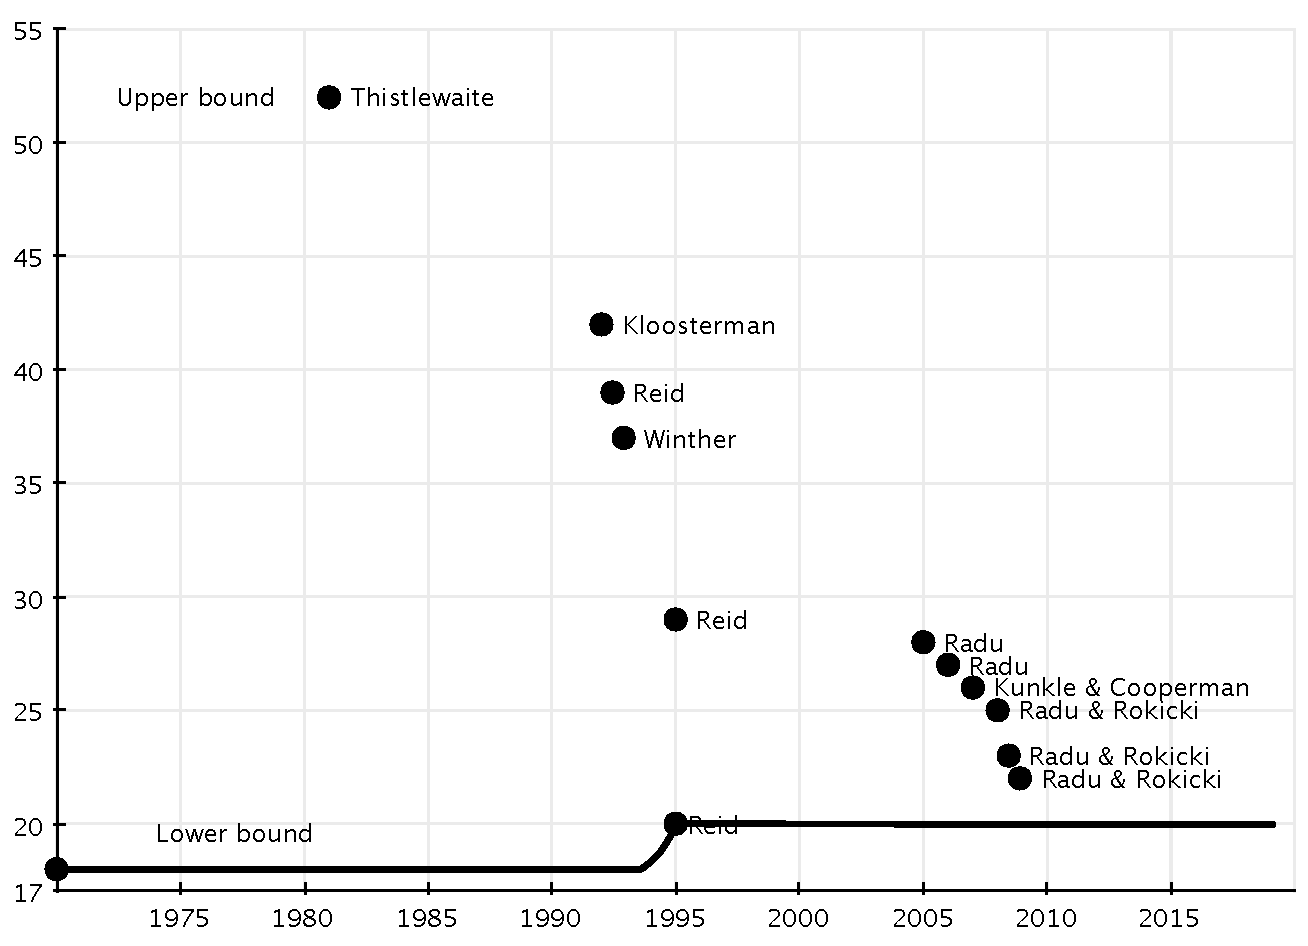
\includegraphics[scale = 0.7]{input/pics/bounds2.pdf}
	\caption{\myCaption{The current upper and lower bound. The x-axis depicts time and y-axis moves.}}
	\label{fig:upperLowerBound}
\end{figure}

\section{The Current and Previous Upper Bounds}
The progression of finding and proving the current and previous upper bounds have been a slow process.
%This is a slow moving field, but some events have occurred in the field the last couple of years.%% DAN DAN DAN DAN giv kilder pl0x
The reason why it is a slow process to prove the upper bound, is that there is a vast amount of different positions a \rubik{} can be in. Even with todays computer power there is simply to much data to process. This have inspired a small group of people to dedicate a lot of time to create and improve algorithms to solve arbitrary \rubik{}s.
%the effect that a small group of people dedicate a lot of time to create and improve algorithms to solve arbitrary \rubik{}s. 

\begin{comment}

The set solver created by Thomas Rockicki, which was described in the previous section will now be further described.

%The result

The set solver has a special way of testing the \rubik{}s. It does not solve them to the unit position $e$, instead it finds a move sequence for a subgroup of the \rubik{} this way it can solve approximately 19.5 billion cubes at a time and not just one. The reason for this is that if you relabel an arbitrary cube, that given cube can be unlabeled to approximately 19.5 billion different cube positions. Recall that there are approximately 19.5 billion positions in the set \m{H} and all these positions are equal to $e$ when relabeled. The same logic applies to any other given position.
\end{comment}

Proofs of the upper bound has been published several times, and it has been lowered each time.
The first to find \textit{God's algorithm} was Thistlethwaite. Thistlethwaite's algorithm was proven to be able to solve an arbitrary \rubik{} in 52 twists or less \cite{jaapthistle}.
\emph{SOMETHING ABOUT HIS ALGORITHM!!!}

This upper bound existed in over 10 years and the next upper bound was found in 1992 by Hans Kloosterman, which reduced the upper bound to 42 moves %\cite{rokickipdf}. 
He modified Thistlethwaite's algorithm and founds some shortcuts to reduce the moves by replacing the \m{G3} subgroup with a different subgroup and removed a move between stage 3 and 4.

In May 1992, Michael Reid reduced the upper bound to 39 moves by using a three phase algorithm and a thorough analysis of the groups.

One day after Michael Reid, Dik Winter reduced the upper bound to 37 moves

\begin{comment}
The progression greatly accelerated when that set solver proved the first upper bound of 25 moves. This was done on home computers from October 2007 to March 2008. They only needed to solve 6000 sets, but after this they got contacted by John Welborn from Sony Pictures Imageworks and he offered a lot of idle computers from a computer farm to help on the project. 
\end{comment}
After this the process of lowering the bound sped up, not long after they proved the upper bound of 24 and 23. As the upper bound is lowered they need to solve more and more sets to ensure that it is the upper bound, and they needed to test almost 27000 and 180000 sets for 24 and 23. 


The current upper bound is on 22 moves and was proved in 2009 \cite{rokicki09}. To prove this they needed to compute 1,265,326 different sets. At the moment they have not proven that the upper bound can be 21, but the computer farm is currently working on it, and they expect that it is possible to lower the upper bound to 20. This means that any arbitrary \rubik{} could be solved in just 20 moves.

\subsection{The Lower Bound}
As mentioned previously in this chapter the lower bound is the number of twists required to solve the \rubik{} in the position which requires the most twists to solve. 
For now it is proven that the superflip position(see figure \ref{fig:superflip}), is the position which requires the most twists to be solved \cite{speedsolving.wiki}.
The shortest path from the superflip to the solved position is 20 twists \cite{rokicki09}.
This has been proven by trying every possible solutions with 19 twists or less. 
There has not been found a position that requires more than 20 twists, which makes the lower bound 20 twists.

\begin{figure}[ht]
	\centering
		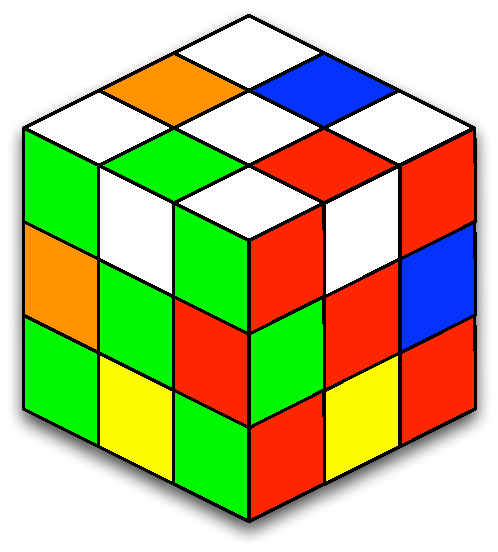
\includegraphics[scale = 0.7]{input/pics/superflip.pdf}
	\caption{\myCaption{The superflip: every edge is flipped. The optimal solution to this position is 20 twists.}}
	\label{fig:superflip}
\end{figure}





\myTail{noget andet}

\myTail{In this chapter it has been described how \erno{} got the idea for the cube. We also stated that \erno{} was not the only one at that time, that came with the invention of cubes. \erno{}'s cube was special since the blocks hold each other together, which is different from the one Doctor Larry D. Nichols applied patent for which is hold together with magnets. 
}
%\end{document}
	%\documentclass{report}\begin{document}
\chapter{Community}
\myTop{In this chapter the community concerning the original \rubik{} and other similar puzzles will be presented and described briefly. This chapter will include a description of the online and offline community and the competitions in which members of the community partake. The community is an important and interesting topic because it is the primary place where solving strategies and algorithms are produced, presented and discussed. 
}

The \rubik{} community consists of both a real life community handling competitions and events and an online community where \cuber{}s can find the real life competitions, improve their skills and talk to each other. The majority of the community is focussed on the speedcubing aspect. In this chapter both the online and offline community will be discussed. Note that the two sides of the community often interfere.

\section{The Online Community}
In the world of the \rubik{} there is a large online community. The community consist of everything from forums and guides to competitions and bragging. \cuber{c}s, as they often refer to them selves as, have a place that is the online community to express and compare their abilities, experiences and skills with each other. 
% Evt. flyt cubers op inden section
\subsection{Forums}
Forums give the \cuber{}s a place for sharing their knowledge and experience\cite{speedsolving.com}\cite{speedcubing.dk}\cite{wca}. Forums or specific \rubik{} sites allow visitors to find information concerning the \rubik{}. The main focus of these forums is on how to solve the \rubik{} or similar puzzles in the least amount of time. Forums are often split into several divisions. Some concerning the hardware used and maintenance techniques for making the \rubik{} spin with greater ease giving the \cuber{} a slightly better solving time.
%Et eller andet med ``some''
A major part is reserved for the theory and the algorithms used to solve the \rubik{} -- most of which strive for an efficient solve both with respect to time and number of \twist{}s.
Another part of the community is focused on competitions of various kinds. The offline competitions are held in cooperation with the World Cube Association(WCA) \cite{wca}, which are further discussed in section \ref{sec:wca}. Beside the WCA-competitions some forums hold weekly online competitions where the forum members can upload and compare their solve times for the \rubik{} or similar puzzles. 

Other than the forums the online community offers a wide variety of sites containing guides, solutions and algorithms for solving the \rubik{}. The majority of the \rubik{} sites contain the beginner's guide\cite{jasminLee08} whose target group is the beginners who may recently have gotten their first cube and want to learn how to solve it. 

\section{Competitions}
\label{sec:wca}
Speed cubing competitions are held on a regular basis\cite{wca/competitions}. These competitions have different disciplines for various puzzles related to the original 3x3x3 \rubik{}. All the official competitions are held in cooperation with the World Cube Association (WCA). The WCA governs the official regulations on speed cubing and holds annual world and regional championships. The first World championship in speed cubing was held in 1982 in Budapest, Hungary. WCA governs the official rankings and records for solving the Rubik's cube. In total WCA keeps regulation, ranking and records for 19 different types of competitions. All 19 competitions include puzzles which are related to or based on the original \rubik{}. 
\myTail{In this chapter the community in regards to the \rubik{} has been described. It has been stated that the community consists of both an online and an offline aspects. In general the strategies and theories are produced and discussed online and they are for one thing put to use in competitions where the right solving method is crucial in order to finish in a competitive time.
}
%\end{document}
	\chapter{Recreational Mathematics}
\label{chap:recreationalMathematics}
\myTop{It is important to understand what recreational mathematics is in order to get a better understanding of the \rubik{}. The \rubik{} is related to other recreational mathematical puzzles, which have inspired the \rubik{} and are simpler to understand at first grasp, than the \rubik{}. This chapter presents a definition of recreational mathematics and a few examples of recreational mathematical puzzles other than the \rubik{}.}
\section{Definition}
Recreation means to do something which is amusing or relaxing. Mathematics is somewhat harder to give a precise definition of, due to the vast amount of subjects that fall under this term. Most people do however have a common idea of what mathematics is.

Recreational mathematics is hereby defined as mathematical problems, puzzles or games which are fun and interesting to laymen. \cite{Singmaster98} \cite[18]{Trigg78}
\section{Puzzles}
This project is dedicated to the \rubik{} and the cube will be covered in detail later in this report. This section will instead describe some puzzles related to the Rubik's cube.

	\subsection{Magic Square}
\label{sec:magicSquare}
A \msquare{} is a square which is divided into a number of subsquares. The number of subsquares on any side is refered to as the ``order'' of that \msquare{}. In each subsquare there is a positive integer. In order for the \msquare{}, to be ``magical'', the sum of any row, column or diagonal must be the same, this sum is refered to as the magic constant.

The \msquare{}\cite{aiden06} originantes from ancient China. It was said that the people near the river Lo made offerings. Every time they made an offering a tortoise emerged from the river. On the back of the tortoise there was said to be a \msquare{}.

The \msquare{} from this tale was a 3 order \msquare{}. This is not the only order in which a \msquare{} can be created; it is possible to make an ``$n$'' order \msquare{}. Although it has been proven that it is not possible to make a second order \msquare{}.

In order to solve the \msquare{}, it is needed to know the magic constant -- the constant which every row, line and diagonal adds up to for the given order $n$. This constant can be computed with the formula in \ref{align:magicConstant}.

\begin{align}
\label{align:magicConstant}
	M(n) = \frac{n \cdot (n^2+1)}{2}
\end{align}

The proof of this formula is quite straight forward. As the table \ref{tab:magicSquareOrder3} illustrates, a \msquare{} of the order 3 contains the numbers from 1 to 9. Generally a \msquare{} of the order $n$ contains the numbers from 1 to $n^2$.

The sum of the numbers of a row in a \msquare{} is equal to the magic constant. If the magic constant is multiplied by the order $n$ it would be equal to the sum of alle the integers, since each number only occurs once in a \msquare{}.

\renewcommand{\arraystretch}{1.3}
\begin{table}[h]
	\centering
		\begin{tabular}{|c|c|c |@{\vrules}| c|}
			\hline
			6&1&8&15 \\
			\hline
			7&5&3&15 \\
			\hline
			2&9&4&15 \\
			\noalign{\hrules}
			15&15&15&45 \\
			\hline
		\end{tabular}
	\caption{\myCaption{A \msquare{} of the order 3, by adding the three numbers in any row, column or diagonal, the magic constant is seen to be 15}}
	\label{tab:magicSquareOrder3}
\end{table}

The equation \ref{proof:magicConstant1} can be rewritten into the equation \ref{proof:magicConstant2}(See proof of the right hand side transcription in appendix X).

\begin{align}
\label{proof:magicConstant1}
	n \cdot M \left( n \right) = \sum ^{n^2}_{i = 1} i = 1 + \cdots + n^2
\end{align}
\begin{align}
\label{proof:magicConstant2}
	n \cdot M \left( n \right) = \frac{n^2 \cdot \left( n^2 + 1 \right)}{2} \\
\label{proof:magicConstant3}
	M \left( n \right) = \frac{n \cdot \left( n^2 + 1 \right)}{2} 
\end{align}

The equation \ref{proof:magicConstant3} shows the function which gives the magic constant for a \msquare{} of the order $n$.

Variations of the \msquare{} exists. For example the numbers which can be inserted into the subsquares, could exeed $n^2$. This would change the magic constant. A \msquare with the intergers 1 to $n^2$ within its subsquares is called a ``Normal \msquare''. %input/introduction/recreationalMathematics/magicSquare %Denne sti skal bruges n�r rapporten samles!
	\subsection{Magic Cube}
\label{sub:mcube}



%\begin{figure}[h]	\centering		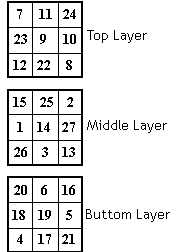
\includegraphics[scale=0.8]{input/pics/presentMagicCube2}	\caption{\myCaption{This is a magic cube split up into 3 magic squares.}}	\end{figure}



\begin{figure}[b]
	\centering
		\subfloat[\myCaption{Top layer.}]{
		
		\begin{tabular}{|c|c|c|}
			\hline
			7&11&24 \\ \hline
			23&9&10 \\ \hline
			12&22&8 \\ \hline
		\end{tabular}
		}
		\hspace{0.02\textwidth}
		\subfloat[\myCaption{Middle layer.}]{
		\begin{tabular}{|c|c|c|}
			\hline
			15&25&2 \\ \hline
			1&14&27 \\ \hline
			26&3&13 \\ \hline
		\end{tabular}

		}
		\hspace{0.02\textwidth}
		\subfloat[\myCaption{Buttom layer.}]{ 
		\begin{tabular}{|c|c|c|}
			\hline
			20&6&16 \\ \hline
			18&19&5 \\ \hline
			4&17&21 \\ \hline
		\end{tabular}
		}
		\caption{\myCaption{This is a magic cube split up into 3 magic squares.}}
		\label{fig:presentMagicCube}
\end{figure}



Both a \msquare{} and a \mcube{} have a magic constant, which can be the sum of each row, column and pillar. See figure \ref{fig:presentMagicCube}.
 However this is where the similarity ends. There are also similarities between the \mcube{} and the \rubik{} which will be elaborated on later. 

We have shown how to calculate the magic constant in a \msquare{}.
In a  \mcube{} there is not a big difference in the formula to calculate the magic constant.
\begin{equation}
	M(n)=\frac{n \cdot (n^3+1)}{2}
\end{equation}
As shown in the formula the only difference is the power of $n$ that is changed from 2 to 3.
See appendix \ref{sec:proofOfMagicConstant} for an explanation.

To create a  \mcube{}, there are some parts that need to be explained.
All these basics are shown on figure \ref{fig:cubeparts}.

\begin{figure}[htb]
	\centering
		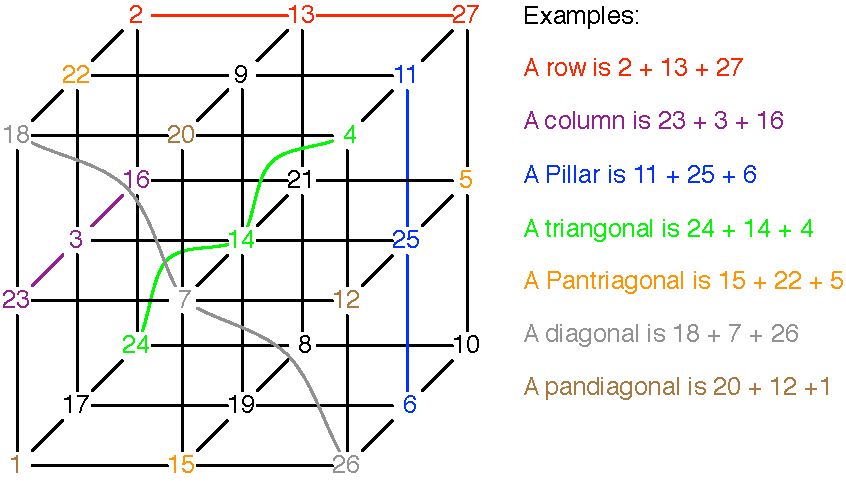
\includegraphics[scale=0.5]{input/pics/cubeparts.pdf}
	\caption{\myCaption{This is a Magic Cube where the colors show all of the parts.}}
	\label{fig:cubeparts}
\end{figure}

Because of all these different parts there are a lot of different ways to define  \mcube{}s.
The simplest of them all is a simple  \mcube{}. The only requirements to make such a cube is the following:
\begin{itemize}
	\item All 9 rows, columns and pillars must be equal to the magic constant.
	\item All 4 triagonals must also equal the magic constant.
\end{itemize}

\begin{figure}[htb]
	\centering
		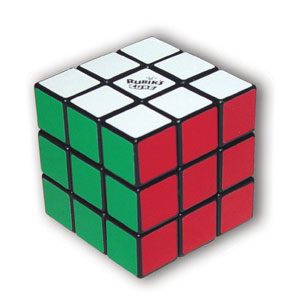
\includegraphics[scale=0.4]{input/pics/rubiksCube}
	\caption{\myCaption{This is a Rubik's Cube.}}
	\label{fig:rubiksCube}
\end{figure}

When looking at the \rubik{} it is easy to see that it looks a lot like the \mcube{}. 
There are two differences. 
The first is that the \mcube{} consists of numbers whereas the \rubik{} has colors, which are different on each \face{}.
The other difference is that the \mcube{} has a number in the center where the \rubik{} center is invisible and out of importancy. This \mcube{} should not be confused with the later presented \mcube{} made by \erno{}.
 %input/introduction/recreationalMathematics/magicCube %Denne sti skal bruges n�r rapporten samles!
	\subsection{Magic Puzzle}
The \mpuzzle{} is also known as the 15-puzzle \cite[pp. 48-50]{Larsen81}. It is a puzzle that consists of a tray with 15 square tiles and an empty square arranged in a 4x4 contraption.

It has never been discovered who actually invented the \mpuzzle{}, but Samuel Loyd who was an American chess player and puzzle author claimed that he invented the \mpuzzle{} and therefore he got the credit. This is turned down by a research of Jerry Slocum. He discovered that there was a wooden version of the game already in 1865, this was manufactured by the Embossing Co. Jerry Slocum searched for the patent and found it, US 50.608 and was applied by a Henry May. 

Jerry Slocum also found a patent by Ernest U. Kinsey that was published August 20th 1878. This version by Ernest U. Kinsey was a 6x6 version of the puzzle which also prevented the tiles from being lifted out.

\subsubsection {Permutations}
The tiles in a \mpuzzle{} can be arranged in $16!$ different positions \cite{jaapsch}. This limit can not be reached because you have to make a permutation to switch the tiles. The permutation must be an even or odd number of transpositions depending on where the position of the empty square is.

The tiles are often numbered or labeled with small pictures which when assembled correctly form a larger picture.

\begin{figure}[htb!]%
	\center
	\subfloat[\myCaption{Figure of Magic Puzzle.}]{\label{fig:MagicPuzzle}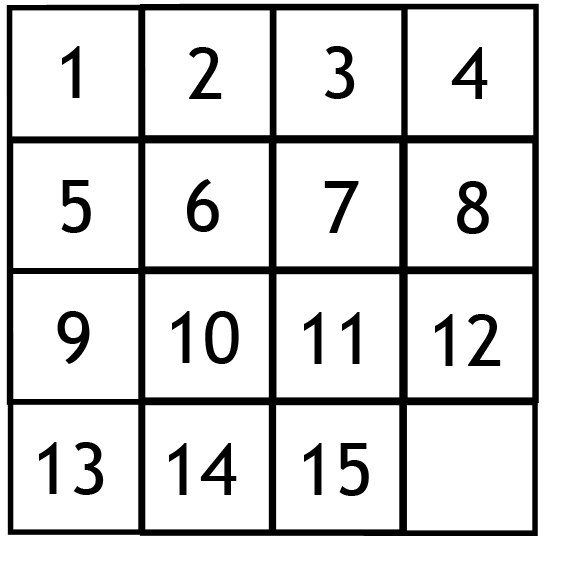
\includegraphics[scale=0.2]{input/pics/MagicPuzzle.png}}
	\hspace{0.02\textwidth}
	\subfloat[\myCaption{Figure of Magic Puzzle with inverse numbers.}]{\label{fig:MagicPuzzleInverse}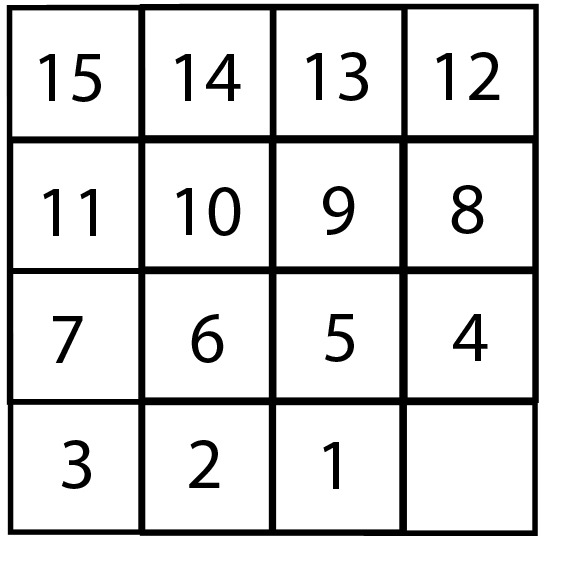
\includegraphics[scale=0.2]{input/pics/MagicPuzzle15-1}}
	\caption{\myCaption{Illustrations of the legal and illegal permutations of the Magic Puzzle.}}
	\label{fig:mpuzzles}
\end{figure}

\begin{comment}
	\begin{figure}[!h]
	\begin{center}
	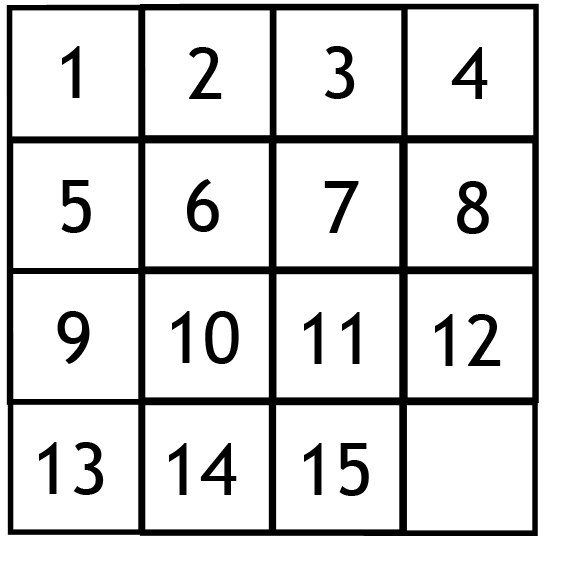
\includegraphics[scale=0.2]{input/pics/MagicPuzzle.png}
	\caption{\myCaption{Figure of Magic Puzzle.}}
	\label{fig:MagicPuzzle}
	\end{center}
	\end{figure}
	
	\begin{figure}[!h]
	\begin{center}
	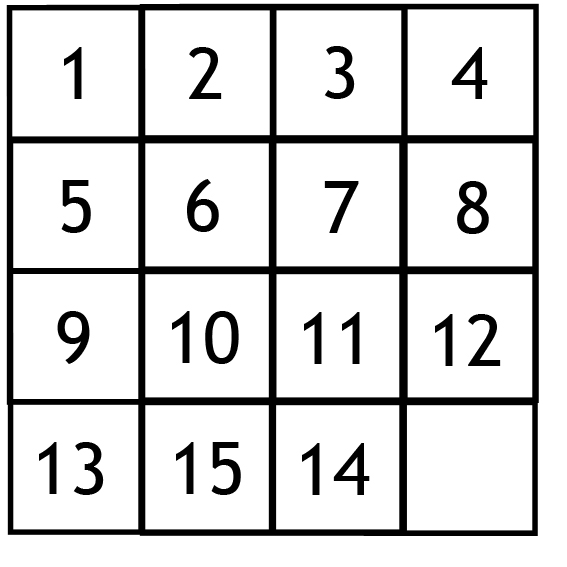
\includegraphics[scale=0.2]{input/pics/MagicPuzzle15-14.jpg}
	\caption{\myCaption{Figure of Magic Puzzle with inverse numbers.}}
	\label{fig:MagicPuzzleInverse}
	\end{center}
	\end{figure}
\end{comment}

For instance we got the figure \ref{fig:MagicPuzzle} and want to switch the tiles to be positioned like on figure \ref{fig:MagicPuzzleInverse} \cite[pp. 48-50]{Larsen81}. This permutation requires an odd transposition of the seven pairs (1,15), (2,14), (3,13), (4,12), (5,11), (6,10) and (7,9). This permutation is not possible because it requires an even number of transpositions to get the empty square at the same position. If we color the contraption like a chess board (see figure \ref{fig:Chess}) we can see that every odd transposition makes the empty square change color and with every even transposition the empty square lands on a square of the same color.

\textit{Did we put in the right picture in \ref{fig:MagicPuzzleInverse}?}

\begin{figure}[!h]
\begin{center}
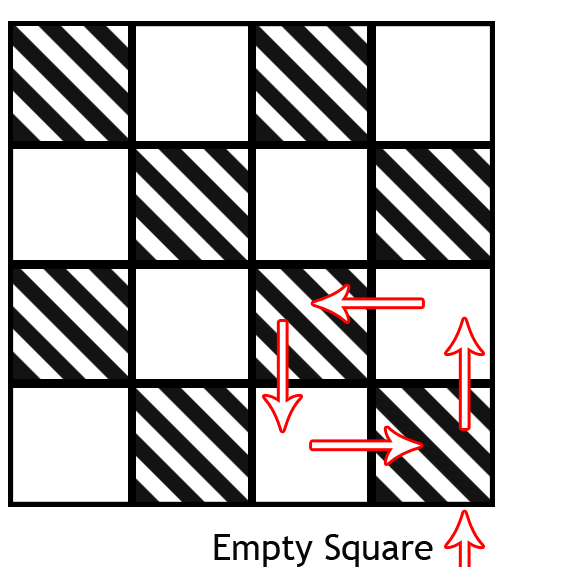
\includegraphics[scale=0.2]{input/pics/MagicPuzzle(EmptySquare).png}
\caption{\myCaption{Figure of Empty Square.}}
\label{fig:Chess}
\end{center}
\end{figure}

Therefore the number of different positions is $\frac{16!}{2}$. But if the empty square has to be in a fixed position then the possible permutations is $\frac{15!}{2}$. These permutations are almost like the ones the \rubik{} uses and they actually inspired \erno{} into his creation of the \rubik{} \cite[pp. 7-9]{Rubik87}. %input/introduction/recreationalMathematics/magicPuzzle %Denne sti skal bruges n�r rapporten samles!
\myTail{This chapter has given a definition of recreational mathematics and shown three puzzles, which all relates to the \rubik{}; \msquare{}, \mcube{} and \mpuzzle{}. The \msquare{} was the predecessor to \mcube{}, which is in turn the predecessor to the \rubik{}. The permutation from the \mpuzzle{} inspired the creation of \rubik{}, which uses a similar principle for moving the \cpiece{}s around.}